%% Preambulo
\documentclass{article}
\usepackage{pgfplots}
\usepackage{lipsum}
\usepackage{filecontents}

%% Ajustes
% PGFPlots settings
% Para mejorar la compatibilidad
\pgfplotsset{compat=1.14}
\usepgfplotslibrary{patchplots}

% Custom fules from filecontents
\begin{filecontents}{datasample.dat}
x y
1 1
2 4
3 9
4 16
5 25
6 36
\end{filecontents}

%% Comandos


%% Documento
\begin{document}
    \lipsum[1]
    \begin{figure}[!h]
        \centering
        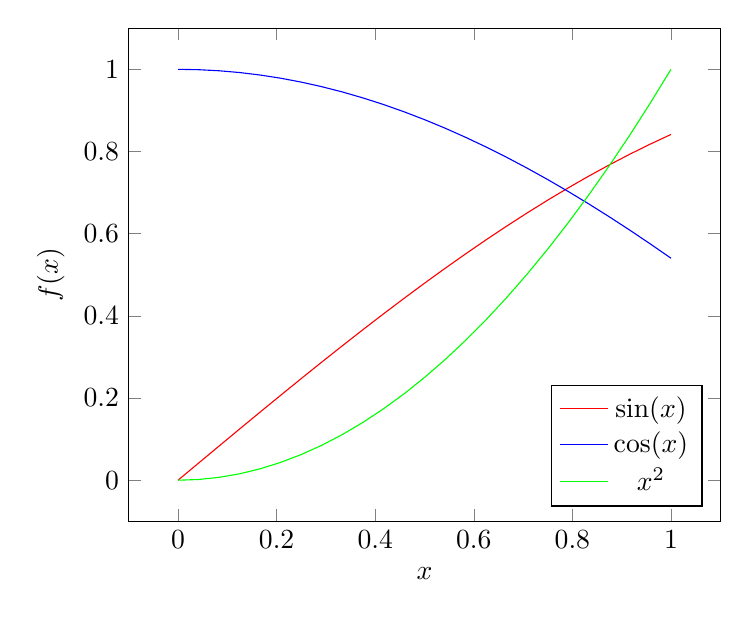
\begin{tikzpicture}
            \begin{axis}[
                    width=0.75\textwidth,
                    domain=0:1,
                    legend pos=south east,
                    ylabel={$f(x)$},
                    xlabel={$x$},
                ]
                \addplot[
                    no markers,
                    color=red
                ]{sin(deg(x))};
                \addplot[color=blue]{cos(deg(x))};
                \addplot[color=green]{x^2};
                \legend{$\sin(x)$, $\cos(x)$, $x^2$}
            \end{axis}
        \end{tikzpicture}
    \end{figure}

    \lipsum[2]

    \begin{figure}[!h]
        \centering
        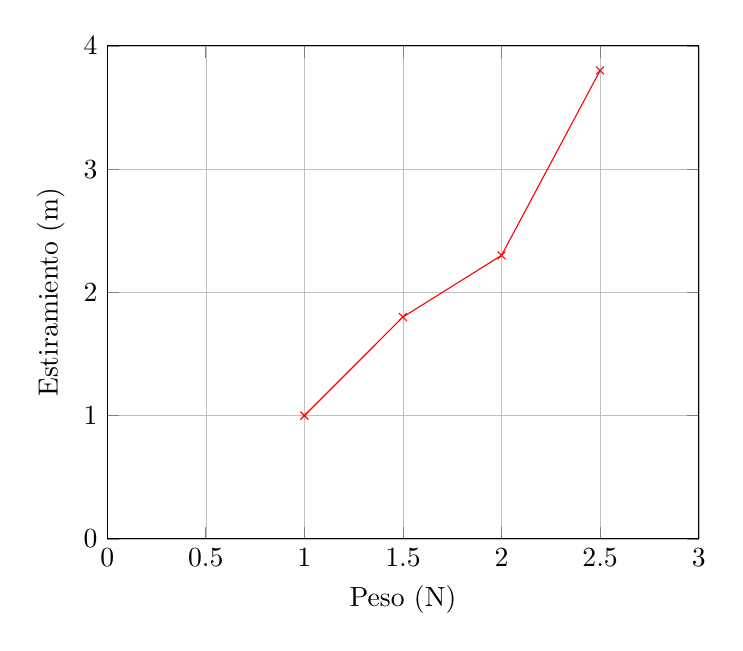
\begin{tikzpicture}
            \begin{axis}[
                    width=0.75\textwidth,
                    xmin=0,
                    xmax=3,
                    ymin=0,
                    ymax=4,
                    grid=major,
                    major grid style={
                        line width=.1pt,
                        draw=gray!50,
                    },
                    scale=1,
                    legend pos=south east,
                    ylabel={Estiramiento (m)},
                    xlabel={Peso (N)},
                ]
                \addplot[
                    mark=x,
                    color=red
                ] coordinates {
                    (1.0, 1.0)
                    (1.5, 1.8)
                    (2.0, 2.3)
                    (2.5, 3.8)
                };
            \end{axis}
        \end{tikzpicture}
    \end{figure}

    \lipsum[3]

    \begin{figure}[!h]
        \centering
        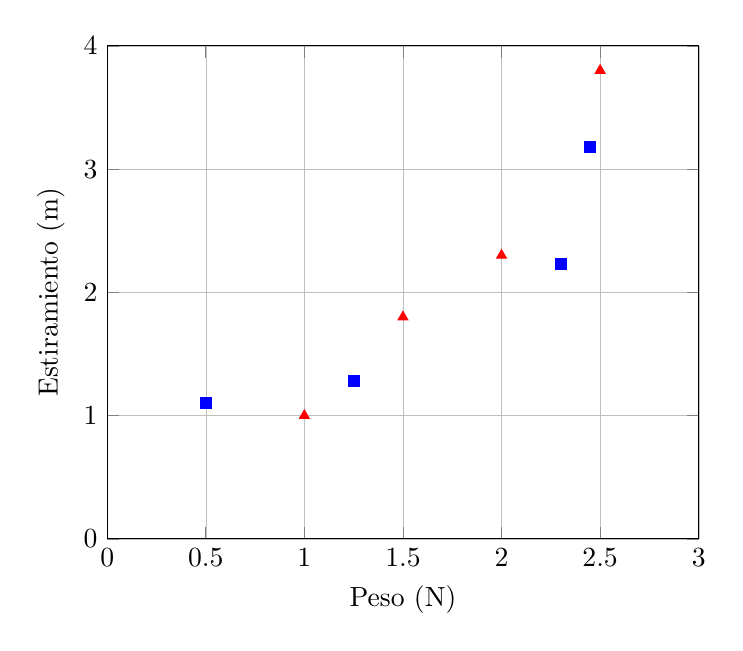
\begin{tikzpicture}
            \begin{axis}[
                    width=0.75\textwidth,
                    xmin=0,
                    xmax=3,
                    ymin=0,
                    ymax=4,
                    grid=major,
                    major grid style={
                        line width=.1pt,
                        draw=gray!50,
                    },
                    scale=1,
                    legend pos=south east,
                    ylabel={Estiramiento (m)},
                    xlabel={Peso (N)},
                ]
                \addplot[
                    only marks,
                    mark=triangle*, % * full filled markers
                    color=red,
                ] coordinates {
                    (1.0, 1.0)
                    (1.5, 1.8)
                    (2.0, 2.3)
                    (2.5, 3.8)
                };
                \addplot[
                    only marks,
                    mark=square*, % * full filled markers
                    color=blue,
                ] coordinates {
                    (0.5, 1.10)
                    (1.25, 1.28)
                    (2.30, 2.23)
                    (2.45, 3.18)
                };
            \end{axis}
        \end{tikzpicture}
    \end{figure}

    \lipsum[3]

    \begin{figure}[!h]
        \centering
        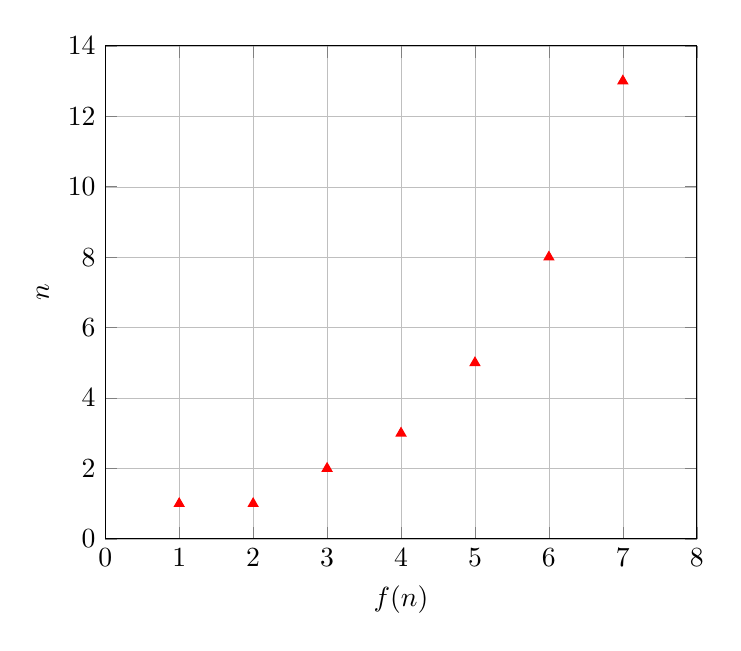
\begin{tikzpicture}
            \begin{axis}[
                    width=0.75\textwidth,
                    xmin=0,
                    xmax=8,
                    ymin=0,
                    ymax=14,
                    grid=major,
                    major grid style={
                        line width=.1pt,
                        draw=gray!50,
                    },
                    scale=1,
                    legend pos=south east,
                    ylabel={$n$},
                    xlabel={$f(n)$},
                ]
                \addplot [
                    only marks,
                    mark=triangle*,
                    color=red,
                ] table [
                    x=n,
                    y=fn
                ]{
                    n    fn
                    1    1
                    2    1
                    3    2
                    4    3
                    5    5
                    6    8
                    7    13
                };
            \end{axis}
        \end{tikzpicture}
    \end{figure}

    \lipsum[3]

    \begin{figure}[!h]
        \centering
        \pgfplotstableread{datasample.dat}{\datasample}
        \begin{tikzpicture}
            \begin{axis}[
                    width=0.75\textwidth,
                    xmin=0,
                    xmax=7,
                    ymin=0,
                    ymax=40,
                    grid=major,
                    major grid style={
                        line width=.1pt,
                        draw=gray!50,
                    },
                    scale=1,
                    legend pos=north west,
                    ylabel={$n$},
                    xlabel={$f(n)$},
                ]
                \addplot [
                    only marks,
                    mark=triangle*,
                    color=red,
                ] table [
                    x=x,
                    y=y,
                ]{\datasample};
                \addlegendentry{Experimental Data}

                \addplot [
                    color=green,
                ] table [
                    x=x,
                    y=y,
                ]{datasample.dat};
                \addlegendentry{Control Data}

                \addplot [
                    color=red
                ] {x^2};
                \addlegendentry{Fit}

            \end{axis}
        \end{tikzpicture}
    \end{figure}

    \lipsum[5]

    \begin{figure}[!h]
        \centering
        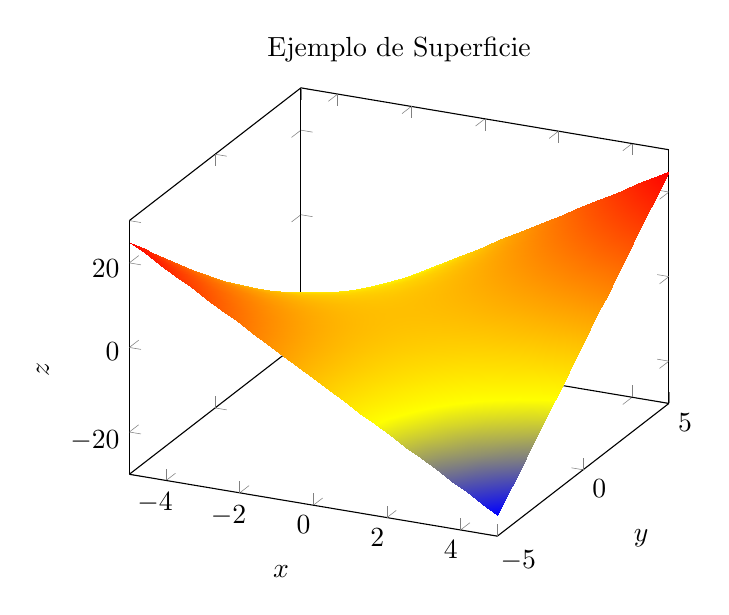
\begin{tikzpicture}
            \begin{axis}[
                    title=Ejemplo de Superficie,
                    xlabel=$x$,
                    ylabel=$y$,
                    zlabel=$z$,
                ]
                \addplot3 [
                    surf,
                    shader=interp,
                    patch type=rectangle,
                ] {x*y};
            \end{axis}
        \end{tikzpicture}
    \end{figure}

    \lipsum[5]

    \begin{figure}[!h]
        \centering
        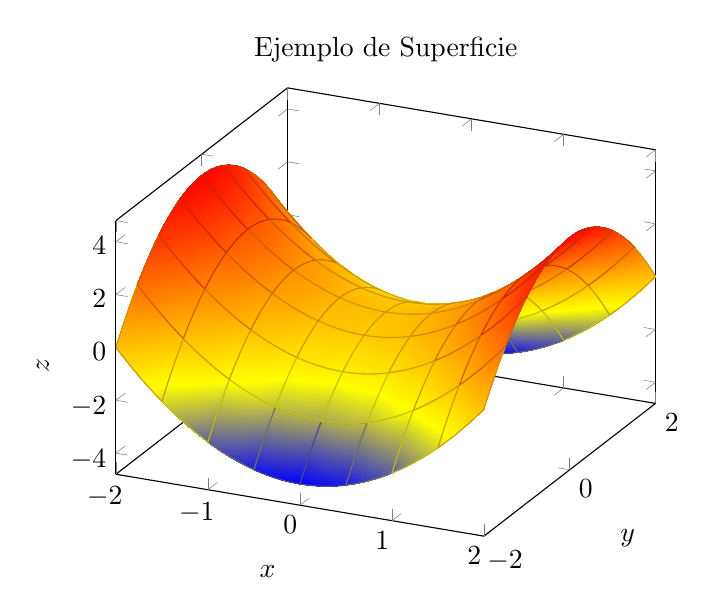
\begin{tikzpicture}
            \begin{axis}[
                    title=Ejemplo de Superficie,
                    xlabel=$x$,
                    ylabel=$y$,
                    zlabel=$z$,
                ]
                \addplot3 [
                    patch,
                    patch refines=3,
                    shader=faceted interp,
                    patch type=biquadratic,
                ] table [
                    z expr=x^2 - y^2,
                ] {
                    x    y
                    -2  -2
                    2  -2
                    2  2
                    -2 2
                    0  -2
                    2  0
                    0  2
                    -2  0
                    0  0
                };
            \end{axis}
        \end{tikzpicture}
    \end{figure}
\end{document}
